%************************************************
\chapter{An Interesting Curve}
%************************************************
\begin{flushright}
October 5, 2012
\end{flushright}
\section{Objective}
	To create an interesting curve and describe why it is interesting.

\section{Approach}
	After substantial thought and consideration of a variety of different definitions for `interesting', I finally decided to create a parametric equation for the letter `A'. To achieve this, I realized it was sufficient to device a method that could combine different `curves'\footnote{The word curve here implies its English meaning. The mathematically precise definition is given later} , which could then be used to make different segments of the letter, to produce a single equation for the same.
	\par
	However, while developing this method, I ended up created something more elegant than the alphabet in itself, which is displayed after the discussion.

\section{Definitions}
	I've used the following functions for constructing the interesting curve. They are needed to crop known parametric curves, to enable the possibility of creating their combinations to get the right shape.
	\par
	The interesting curve is given by 
	\begin{equation}
		\gamma : (\alpha,\beta) \rightarrow \mathbb R^{3}
	\end{equation}
		\subsection{Left Crop Function}
			The Left Crop Function is defined as
			\begin{equation}
				C_L(t,c) = \lceil m (t - c) \rceil
				\label{left}
			\end{equation}
			where $t$ is the parameter of the interesting curve, $c$ is a constant $\in \mathbb R$, chosen s.t. before it, a function multiplied to $C_L(t,c)$ is cropped and $m$ is a small constant $\in \mathbb R$, s.t. $C_L(\alpha,c)=0$ and $C_L(\beta,c)=1$.
		\subsection{Right Crop Function}
			The Right Crop Function is defined as
			%\lceil m (-t + c) \rceil
			\begin{equation}
				C_R(t,c) = \lfloor m (-t + b) \rfloor + 1
				\label{left}
			\end{equation}
			where $t$ is the parameter of the interesting curve, $c$ is a constant $\in \mathbb R$, chosen s.t. after it, a function multiplied to $C_R$ is cropped and $m$ is a small constant $\in \mathbb R$, s.t. $C_R(\alpha,c)=1$ and $C_R(\beta,c)=0$.

		\subsection{Centre Crop Function}
			The Centre Crop Function is defined as
			\begin{equation}
				C_C(t,c_1,c_2) = C_L(t,c_1)C_R(t,c_2) = (\lceil m (t - c_1) \rceil)(\lfloor m (-t + c_2) \rfloor + 1)
				\label{left}
			\end{equation}
			where $t$ is the parameter of the interesting curve, $c_1$, $c_2$ are constants $\in \mathbb R$, chosen so that outside $(c_1,c_2)$, a function is cropped; and $m$ is a small constant $\in \mathbb R$, s.t. $C_C(\alpha,c_1,c_2)=0$ and $C_C(\beta,c_1,c_2)=0$.
			\par
			Observe that $C_C(c_1,c_1,c_2)=0$ while $C_C(c_2,c_1,c_2)=1$. This is a result of carefully defined Left and Right Crop Functions, whose product yields this property. This property is essential for combining multiple curves, as shall become obvious shortly.

		\subsection{Bracket Curve}
			Let $\gamma: (\alpha,\beta) \rightarrow \mathbb R^3$. If $\gamma(\alpha)$ exists, then the given curve, $\gamma$ is a Bracket Curve.

		\subsection{Base Curve}
			Let $\gamma: (\alpha,\beta) \rightarrow \mathbb R^3$. If $\gamma$ is a bracket curve with $\alpha=0$ and $\beta=\infty$ , then the curve is said to be a Base Curve.

		\subsection{Scalar Multiplication Notation}
			Let $\gamma: (\alpha,\beta) \rightarrow \mathbb R^3$ be given by $(\gamma_x(t),\gamma_y(t),\gamma_z(t))$. Let $s(t) \in \mathbb R^3$ be a scalar function of $t$. Then $s(t)\gamma$ is defined to be\\
			$(s(t)\gamma_x(t),s(t)\gamma_y(t),s(t)\gamma_z(t))$.

\section{Generic Curve Extension Algorithm}
	The objective is to create a curve $\gamma : (0,\beta) \rightarrow \mathbb R^3$, by combining $N$ base curves. Assume we have already combined $n-1$ base curves (how exactly, we do not care at this stage) to obtain another base curve given by
	\begin{equation}
		\gamma_{n-1}:(0,t_{n-1}) \rightarrow \mathbb R^3
	\end{equation}
	where $0<t_{n-1}<\beta$.
	\par
	We now wish to extend this curve to $t_n$ s.t. $t_{n-1}<t_n \le \beta$, using a Base Curve $A_n:(0,t_n) \rightarrow \mathbb R^3$. Here we consider two important cases. Let $\gamma_n$ be the extended curve.
	\begin{enumerate}
		\item We wish to start from the origin. For this we define $\gamma_n$ to be
			\begin{equation}
				C_c(0,t_{n-1})\gamma_{n-1}(t) + C_c(t,t_{n-1},t_n)\{A_n(t-t_n-1)\}
			\end{equation}
		\item We wish to start from the point $\gamma_{n-1}(t_{n-1})$. For this we define $\gamma_n$ to be
			\begin{equation}
				C_c(0,t_{n-1})\gamma_{n-1}(t) + C_c(t,t_{n-1},t_n)\{\gamma_{n-1}(t_{n-1}) + A_n(t-t_n-1)\}
			\end{equation}
	\end{enumerate}

\section{Rotational Clone Algorithm}
	Here, using a special case of the Generic Curve Extension Algorithm, we construct a curve that traces rotational clones of a given curve. We set out by defining the following parameters and functions.
	\begin{enumerate}
		\item $k$ represents the number of clones required (about the origin).
		\item $\gamma:(0,\alpha) \rightarrow \mathbb R^3$ represents a base curve which will be cloned.
		\item $C_C(t,c_1,c_2)$ is the centre crop function as defined earlier.
		\item $T_{\theta}$ represents transformation: counter-clockwise rotation by an angle $\theta$ in the X-Y plane.
		\item $\gamma_n (t,\alpha,k)$ is defined to be
		\begin{equation}
			C_C(t,(n-1)\alpha,n\alpha)T_{(n-1)2\pi/k}(\gamma(t - (n-1)\alpha))
		\end{equation}		
	\end{enumerate}
	The final equation will then be
	\begin{equation}
		\gamma_{final} = \sum_{n=1}^k \gamma_n
	\end{equation}

\section{An Interesting Curve}
	Following from the previous section, if we define $k=5$, $\alpha=5$, $\gamma(t)=((t)(1.2^t)cos(t)),((t)(1.2^t)sin(t))$ we get \autoref{aic2}, which is another interesting curve.
	\\
	And just to add some more flavour, if we change the second $1.2$ to $1.1$, and make $\alpha=20$, we obtain \autoref{aic3}.\\	

	% \begin{figure}[bth]
	% 	\begin{center}
	% 		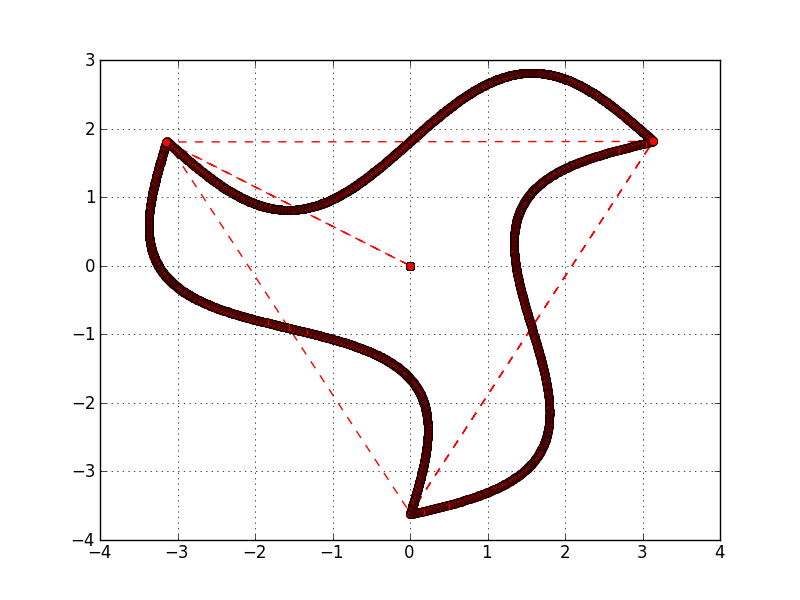
\includegraphics[width=0.9\linewidth]{img/sin_clone}
	% 	\end{center}
	% \caption[An Interesting Curve]{An Interesting Curve}
	% \label{aic}
	% \end{figure}

	\begin{figure}[bth]
		\begin{center}
			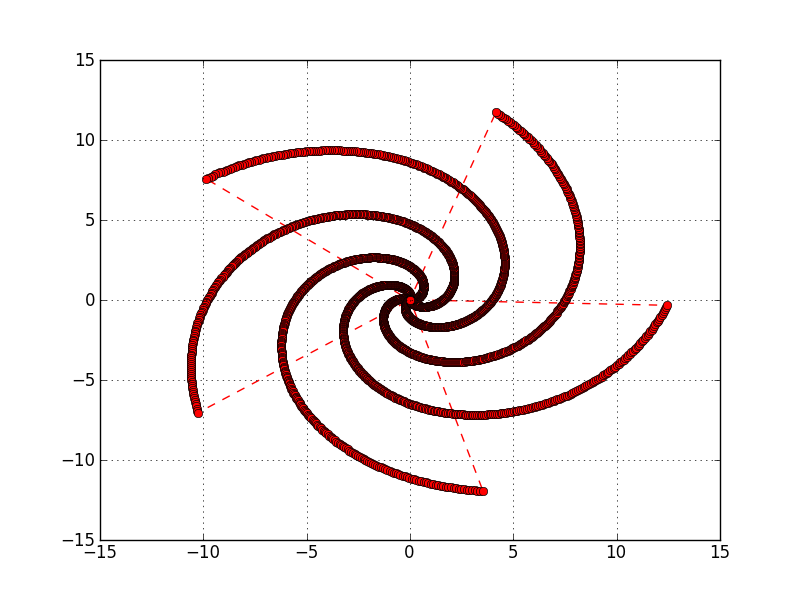
\includegraphics[width=0.9\linewidth]{img/spiral_lessdense_clone.png}
		\end{center}
	\caption[Another Interesting Curve]{Another Interesting Curve}
	\label{aic2}
	\end{figure}

	\begin{figure}[bth]
		\begin{center}
			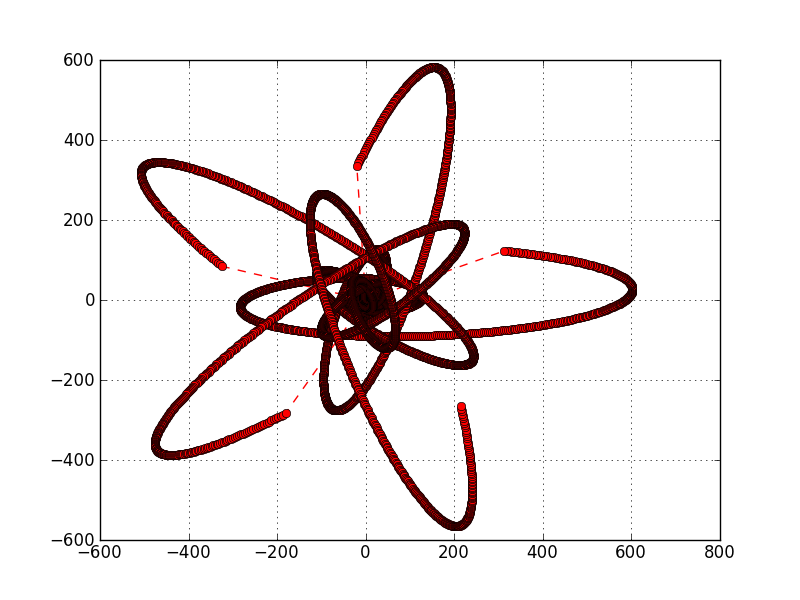
\includegraphics[width=0.9\linewidth]{img/spiral_lessdense2_clone}
		\end{center}
	\caption[Yet Another Interesting Curve]{Yet Another Interesting Curve}
	\label{aic3}
	\end{figure}

\section{Acknowledgements}
	I would like to sincerely acknowledge the contribution of my dear friend, Arjit Kant Gupta, as it was he who came up with the trace of the curves in the first place.

\section{Implementation}
	The curves were created using Python 2.7 and Matplotlib. The source code and this very document are available in the repository provided in the colophon.